\documentclass[11pt]{scrartcl}
\usepackage[utf8]{inputenc}
\usepackage{amsmath, amssymb, amsthm, bbm}
\usepackage{booktabs, verbatim, graphicx, framed}
\usepackage[sexy, hints]{evan}
\begin{asydef}
  defaultpen(fontsize(9pt));
  pointfontsize = 9;
  markscalefactor=0.01;
\end{asydef}
\title{My Favorite Olympiad Problems!}
\author{Anay Aggarwal}
\begin{document}

\maketitle
\section{Introduction}
These are my favorite olympiad problems! I have only done a few, and they are all "beginner" problems.
\section{Algebra}
Algebra is the best.
\begin{example}
  [IMO SL, 1967]
  If $x,y,z$ are real numbers satisfying relations
  \[x+y+z = 1 \quad \textrm{and} \quad \arctan x + \arctan y + \arctan z = \frac{\pi}{4},\]
  prove that $x^{2n+1} + y^{2n+1} + z^{2n+1} = 1$ holds for all positive integers $n$.
\end{example}
\begin{soln}
  Summing the arctans with the formula,

  $$\arctan\left(\frac{x+y+z-xyz}{1-(xy+yz+xz)}\right)=\frac{\pi}{4}$$
  $$x+y+z-xyz=1-(xy+yz+xz)$$
  $$xyz=xy+yz+xz$$

  So $x,y,z$ are roots of $t^3-t^2+kt-k=0$, where $k=xyz=xy+yz+xz$. This factors
  as $(t^2+k)(t-1)=0$. So the roots are $1, \sqrt{-k}, -\sqrt{-k}$, from which the
  result comes immediately.

\end{soln}
\begin{example}
  [Iran 2007, Round 3]
  Let $ a,b$ be two complex numbers. Prove that roots of $ z^{4}+az^{2}+b$ form a rhombus with origin as center, if and only if $ \frac{a^{2}}{b}$ is a non-positive real number.
\end{example}
\begin{soln}
  First of all, the vertices are of the form $t, -t, p, -p$. It's a rhombus if and only if $p=rit$ for some real $r$.
  Notice that there must exist some complex numbers $t, r$ such that
  $$z^4+az^2+b=(z^2-t^2)(z^2+r^2t^2)$$
  And then $a=t^2(r^2-1), b=-r^2t^4$. Hence $\frac{a^2}{b}=-\left(\frac{r^2-1}{r}\right)^2$, which is non-positive real
  if and only if $r\in\mathbb{R}$, i.e. $p=rit$, done.

\end{soln}
\begin{example}
  [Putnam 1971]
  Find all polynomials $f(x)$ such that $f(0)\equiv 0$ and $f(x^2+1)=[f(x)]^2+1$
\end{example}
\begin{soln}
  The answer is only $f\equiv \mathrm{id}$. Let $S$ be the set of numbers $x$ such that $f(x)=x$. It suffices to show that the
  cardinality of $S$ is infinite.

  Suppose for the sake of contradiction that $S$ has finite cardinality. Due to
  the fact that $f(0)=0$, $S\ne \emptyset$. Then it is valid to let $k$ be the maximum
  element found in $S$. Notice that $f(k^2+1)=f(k)^2+1=k^2+1$, thus $k^2+1\in S$, contradiction.
\end{soln}
\begin{example}
  [USAMO 1975]
  If $ P(x)$ denotes a polynomial of degree $ n$ such that $ P(k)=\frac{k}{k+1}$ for $ k=0,1,2,\ldots,n$, determine $ P(n+1)$.
\end{example}
\begin{soln}
  Let $Q(k)=(k+1)P(k)-k$. Hence for $k=0,1,2,\cdots, n$, $Q(k)=0$. Therefore, we can let
  $$Q(x)=c\prod_{i=0}^{n}(x-i)$$
  For a constant $c$. Notice that $Q(-1)=1$, hence
  $$-1=c\prod_{i=0}^n (-i-1)=c(-1)^{n+1}(n+1)!$$
  $$c=\frac{1}{(-1)^{n+1}(n+1)!}$$
  And hence $Q(n+1)=\frac{1}{(-1)^{n+1}}=(n+2)P(n+1)-(n+1)$ thus
  $$\boxed{P(n+1)=\frac{n+1+(-1)^{1-n}}{n+2}},$$
  or if you desire a piecewise representation:
  $$\boxed{P(n+1)=\begin{cases}1 & n\equiv 1 \pmod{2} \\ \frac{n}{n+2} & n\equiv 0 \pmod{2}\end{cases}}$$
\end{soln}
\begin{example}
  [IMO 1963]
  Prove that $\cos{\frac{\pi}{7}}-\cos{\frac{2\pi}{7}}+\cos{\frac{3\pi}{7}}=\frac{1}{2}$.
\end{example}
\begin{soln}
  Let $\omega=\mathrm{cis}\left(\frac{\pi}{14}\right)$. Thus it suffices to show that $\omega+\omega^{-1}-\omega^2-\omega^{-2}+\omega^3+\omega^{-3}=1$. Now using the fact that $\omega^k=\omega^{14+k}$ and $-\omega^2=\omega^9$, this is equivalent to\[\omega+\omega^3+\omega^5+\omega^7+\omega^9+\omega^{11}+\omega^{13}-\omega^7\]\[\omega\left(\frac{\omega^{14}-1}{\omega^2-1}\right)-\omega^7\]But since $\omega$ is a $14$th root of unity, $\omega^{14}=1$. The answer is then $-\omega^{7}=1$, as desired.
\end{soln}
\begin{example}
  [JMMO]
  Let $x$, $y$ and $z$ be positive real numbers such that $x+y+z = 1$. Prove the inequality:

  $$\frac{x^2}{1+y}+\frac{y^2}{1+z} +\frac{z^2}{1+x} \leq 1$$
\end{example}
\begin{soln}
  Notice that $x<1-y<1+y$, hence $\frac{x}{1+y}\le 1\to \frac{x^2}{1+y}\le x$. Summing cyclically yields the desired result.
\end{soln}
\begin{example}
  [IMO 1984]
  Prove that $0\le yz+zx+xy-2xyz\le{\frac{7}{27}}$, where $x,y$ and $z$ are non-negative real numbers satisfying $x+y+z=1$.
\end{example}
\begin{soln}
  For the lower bound, $xy+yz+xz-2xyz=(xy+yz+xz)(x+y+z)-2xyz\ge 0$ upon expansion.
  For the upper bound,
  $$2\left(\frac{1}{2}-x\right)\left(\frac{1}{2}-y\right)\left(\frac{1}{2}-z\right)=\frac{1}{4}-\frac{1}{2}(x+y+z)+xy+yz+xz-2xyz$$
  $$xy+yz+xz-2xyz=\frac{1}{4}+2\prod_{cyc}\left(\frac{1}{2}-x\right)$$
  Simple AM-GM on the $\frac{1}{2}-x$ terms gives
  $$\frac{1}{6}\ge \sqrt[3]{\prod_{cyc}\left(\frac{1}{2}-x\right)}$$
  $$\prod_{cyc}\left(\frac{1}{2}-x\right)\le \frac{1}{216}$$
  $$xy+yz+xz-2xyz\le \frac{7}{27}$$
  As desired. AM-GM is allowed, unless suppose that say $x>\frac{1}{2}$.
  In this case, $xy+yz+xz-2xyz\le \frac{1}{4}$, which we don't care about.
\end{soln}
\begin{example}
  [Kyrgyzstan]
  Find all functions $f:\mathbb{R}\to \mathbb{R}$ such that
  $$f(f(x)^2+f(y))=xf(x)+y$$
\end{example}
\begin{soln}
  Asserting $P(0,0)$, there must be some $a$ such that $f(a)=0$.
  Hence assert $P(a,0)$ to get
  $$f(f(y))=y$$
  Thus $f$ is an involution and thus a bijection (well-known, easy to prove).
  Assert $P(f(b), y)$. We then get
  $$f(b^2+f(y))=bf(b)+y$$
  Assert $P(b,y)$. We then get
  $$f(f(b)^2+f(y))=bf(b)+y=f(b^2+f(y))$$
  Remembering that $f$ is a bijection, $[f(b)]^2=b^2$. Hence $f(b)=\pm b$.
  Unfortunately, we now run into the pointwise trap.
  Suppose that $f(x)=x$ and $f(y)=-y$. Thus
  $$f(x^2-y)=x^2+y$$
  Since $f(b)=\pm b$, then $y=0\to f(y)=0=y$, or $x=0\to f(x)=0=-x$.
  The alternative case is isomorphic.
\end{soln}
\begin{example}
  [Titu Andreescu]
  Let $0\le a,b,c,d\le 1$. Prove that
  $$(1-a)(1-b)(1-c)(1-d)+a+b+c+d\ge 1$$
\end{example}
\begin{soln}
  Fix $b,c,d$. Then the left-hand side is a convex function in $a$,
  specifically linear. Hence the minimum is attained at one of the end points.
  Repeating this argument for $b,c,d$ we deduce that in order for the minimum
  to occur, $a,b,c,d\in\{0,1\}$ must hold.
  If at least one of the numbers is $1$, $LHS=a+b+c+d\ge 1$. \\
  If all are zero, it clearly holds true, as desired. \\ \\
  The technique used brushes up on \textit{smoothing}.
\end{soln}
\begin{example}
  [Macedonia 2021]
  Let $x,y,z$ be positive reals such that $xy+yz+xz=27$. Prove that
  $$x+y+z\ge \sqrt{3xyz}$$
\end{example}
\begin{soln}
  It's easy to prove with Cauchy/AM-GM that $x^2+y^2+z^2\ge xy+yz+xz$.
  Hence
  $$(x+y+z)^2=x^2+y^2+z^2+2(xy+yz+xz)\ge 3(xy+yz+xz)$$
  So it suffices to show that $xyz\le 27$. But AM-GM tells us that
  $$27=xy+yz+xz\ge 3\sqrt[3]{(xyz)^2}$$
  Which gives the desired inequality.
\end{soln}
\begin{example}
  [Crux 4698]
  Let $x_1,\cdots,x_n>0$ be real numbers such that $x_1+x_2+\cdots+x_n=1$. Prove that
  $$\sum_{i=1}^{n}x_i\ln(1+x_i)<\ln 2$$
\end{example}
\begin{soln}
  Consider only $n\ge 2$, since it's obvious for $n=1$.
  Take all indices of summations/products to be from $1$ to $n$. Writing the LHS using log rules, it's equivalent to
  $$\prod (1+x_i)^{x_i}<2$$
  Firstly, note that, by Cauchy-Schwarz,
  $$\left(\sum x_i\right)^2\ge n\sum x_i^2$$
  $$\sum x_i^2\le \frac{1}{n}<1$$
  Then we can use Young's inequality to get
  $$\prod (1+x_i)^{x_i}\le \sum x_i(1+x_i)=\sum x_i+\sum x_i^2<2$$
  As desired.
\end{soln}
\begin{example}
  [AMSP Algebra 3.5 Week 2 Test Problem 4/5]
  Show that for any $n\ge 2$ and $a_1,\cdots, a_n>0$ and $0\le x<y$,
  $$\left(\sum_{i=1}^n a_i^x\right)\left(\sum_{i=1}^n a_i^{-x}\right)\le \left(\sum_{i=1}^n a_i^y\right)\left(\sum_{i=1}^n a_i^{-y}\right)$$
\end{example}
\begin{soln}
  This is equivalent to proving that the function
$$f(t)=\left(\sum_{i=1}^n a_i^t\right)\left(\sum_{i=1}^n \frac{1}{a_i^t}\right)$$
is non-decreasing, i.e. $f'(t)\ge 0$ for all $t>0$. By the product rule,
$$f'(t)=\left(\sum_{i=1}^n a_i^t\ln(a_i)\right)\left(\sum_{i=1}^n \frac{1}{a_i^t}\right)-\left(\sum_{i=1}^n a_i^t\right)\left(\sum_{i=1}^n \frac{\ln(a_i)}{a_i^t}\right)$$
Thus we need to show that for all $t>0$
$$\left(\sum_{i=1}^n a_i^t\ln(a_i)\right)\left(\sum_{i=1}^n a_i^{-t}\right)\ge \left(\sum_{i=1}^n a_i^t\right)\left(\sum_{i=1}^n a_i^{-t}\ln(a_i)\right)$$
For simplicity, write this as $S_n\ge P_n$. We will prove this by induction on $n$, but first we need a lemma:
\\ \\
\textbf{Lemma:}  For any positive reals $x$ and $t$,
$$x^t\ln(x)\ge x^{-t}\ln(x)$$
\\ \\
\textbf{Proof:} If $x\ge 1$, it rearranges to $x^{2t}\ge 1$, which is true. If $x<1$, it rearranges to $x^{2t}\le 1$, which is true, as desired.
\\ \\
Now we proceed with the induction. The base case is $n=2$. This simply reduces to our lemma with $x=\frac{a_1}{a_2}$. For the inductive step, we write
$$S_{n+1}=S_n+a_{n+1}^t\ln(a_{n+1})(a_1^{-t}+\cdots+a_n^{-t})+a_{n+1}^{-t}(a_1^t\ln(a_1)+\cdots+a_n^t\ln(a_n))+\ln(a_{n+1})$$
$$P_{n+1}=P_n+a_{n+1}^{-t}\ln(a_{n+1})(a_1^t+\cdots+a_n^t)+a_{n+1}^t(a_1^{-t}\ln(a_1)+\cdots+a_n^{-t}\ln(a_n))+\ln(a_{n+1})$$
Thus we need to show that

$$\ln(a_{n+1})\left(\sum_{i=1}^n \left(\frac{a_{n+1}}{a_i}\right)^t \right)+\sum_{i=1}^n \left(\frac{a_i}{a_{n+1}}\right)^t\ln(a_i)\ge \ln(a_{n+1})\left(\sum_{i=1}^n \left(\frac{a_i}{a_{n+1}}\right)^t\right)+\sum_{i=1}^n \left(\frac{a_{n+1}}{a_i}\right)^t\ln(a_i)$$

This is equivalent to

$$\sum_{i=1}^n \left(\frac{a_{n+1}}{a_i}\right)^t \ln\left(\frac{a_{n+1}}{a_i}\right)\ge \sum_{i=1}^n \left(\frac{a_{i}}{a_{n+1}}\right)^t \ln\left(\frac{a_{n+1}}{a_i}\right)$$

Which is true by our lemma.
\end{soln}
\section{Combinatorics}
Combinatorics is both the life and death of me.
\begin{example}
  [Canada]
  Let there be a fixed positive integer $n$. Find the sum of all integers such that, when represented in base 2, has $2n$ digits, consisting of $n$ ones,
  and $n$ zeroes.
\end{example}
\begin{soln}
  If $n=1$ we can easily get that the sum is $2$.
  For $n\ge 2$, the first digit is one, so there are $\binom{2n-1}{n-1}$ ways to put the 1's in the empty slots. Then $\binom{2n-2}{n-2}$, etc.
  So $\binom{2n-1}{n-1}+\binom{2n-2}{n-2}+...=\binom{2n-1}{n}+\binom{2n-2}{n}+...=\binom{2n-1}{n}2^{2n-1}$. Then there is $\binom{2n-2}{n}$ of other powers of $2$.
  The requested result is
  $$\binom{2n-2}{n}(1+2+2^2+...+2^{2n-2})+\binom{2n-1}{n}2^{2n-1}=\boxed{\binom{2n-2}{n}(2^{2n-1}-1)+\binom{2n-1}{n}2^{2n-1}}$$
\end{soln}
\begin{example}
  [USAJMO 2010]
  Two permutations $a_1,a_2,\dots,a_{2010}$ and $b_1,b_2,\dots,b_{2010}$ of the numbers $1,2,\dots,2010$ are said to intersect if $a_k=b_k$ for some value of $k$ in the range $1\le k\le 2010$. Show that there exist $1006$ permutations of the numbers $1,2,\dots,2010$ such that any other such permutation is guaranteed to intersect at least one of these $1006$ permutations.
\end{example}
\begin{soln}
  \textbf{Construction:} Pick $S\subseteq \{1,2,...,2010\}$ with $|S|=1004$. Let $Q$ be the set of elements in $\{1,2,...,2010\}\notin S$. Clearly $|Q|=1006$.

  Suppose the said permutations are $b_1, b_2,..., b_{1006}$. For each set $\mathcal{A}_i$, pick $\mathcal{A}_{i_n}$ to be the $n$th element in $\mathcal{A}_i$.
  Pick $b_{i_j}=S_{j-1006}\forall 1007\le j\le 2010$. Define the $k$th \textit{loop} of a permutation of $\{1,...,n\}$ to be some $\{k,...,n,1,...,k-1\}$
  with $n\ge k\ge 1$. Set the first $1006$ elements of $b_i$ to be the $i$th \textit{loop} of $Q$.

  \textbf{Proof that the construction is valid:} From pigeonhole, there exists an element $\epsilon$ of $Q$ such that $\epsilon$ is in one of
  $b_{i_j}$ with $1\le j\le 1006$.

  But with our construction, in each of the first $1006$ columns of some $b_i$, each of the numbers in $Q$ exists. Since $\epsilon$ is also an element of $Q$,
  there must be an intersection, so we're done.
\end{soln}
\begin{example}
  [2020 ISL]
  Let $n$ be a positive integer. Find the number of permutations $a_1$, $a_2$, $\dots a_n$ of the
  sequence $1$, $2$, $\dots$ , $n$ satisfying
  $$a_1 \le 2a_2\le 3a_3 \le \dots \le na_n$$.
\end{example}
\begin{soln}
  The answer is the $n+1$th Fibonacci number. I prove this with strong induction.
  Let there be $P(n)$ ways for a sequence of $n$ numbers.
  The base cases are easy since
  $$P(1)=|\{1\}|=1=F_2$$
  $$P(2)=|\{1,2\}, \{2,1\}|=2=F_3$$
  We do casework on the index of $n$. If $n$ is at the last position, there are
  $P(n-1)$ ways. If $n$ is at the second-to-last position, $n-1$ must be at the
  last position, hence there are $P(n-2)$ ways. I now prove that $n$ cannot be
  at any other position, effectively solving the problem.
  \newline \newline
  Suppose the contrary. Clearly, $n$ cannot be at the first position.
  Hence there is a valid sequence of the first $k$ numbers, then $n$,
  then a jumble of the other numbers. Consider the number $k+1$.
  Let's say its at index $r$. Then
  $$n(k+1)\le (k+1)r$$
  $$n\le r$$
  $$r=n$$
  Hence $k+1$ is the last number. Suppose that the number at index $n-1$ is
  $r$. Thus
  $$(n-1)r\le(k+1)n$$
  But $k+2\le r$, hence
  $$(k+2)(n-1)\le (k+1)n$$
  $$nk+2n-k-2\le nk+n$$
  $$n\le k+2$$
  Meaning that there are at least $n-2$ numbers before the number $n$,
  i.e. $n$ is at one of the last two spots, as desired.
\end{soln}
\begin{example}
  [IMO 2021 P5]
  Two squirrels, Bushy and Jumpy, have collected 2021 walnuts for the winter. Jumpy numbers the walnuts from 1 through 2021, and digs 2021 little holes in a circular pattern in the ground around their favourite tree. The next morning Jumpy notices that Bushy had placed one walnut into each hole, but had paid no attention to the numbering. Unhappy, Jumpy decides to reorder the walnuts by performing a sequence of 2021 moves. In the $k$-th move, Jumpy swaps the positions of the two walnuts adjacent to walnut $k$. Prove that there exists a value of $k$ such that, on the $k$-th move, Jumpy swaps some walnuts $a$ and $b$ such that $a<k<b$.
\end{example}
\begin{soln}
  Let's suppose that Jumpy is hungry and eats every walnut they swap the neighbors of before they swap them. Notice that we want to show that
  Jumpy swaps some uneaten walnut with some eaten walnut at some point in time (assume an eaten walnut is just the crumbs).
  Assume the contrary, i.e. they always swaps some two walnuts of the same status.
  \begin{lemma}
    Swapping two walnuts of the same status preserves the number of pairs of adjacent uneaten walnuts.
  \end{lemma}
  This is obvious since swapping two walnuts of the same status doesn't change anything about the statuses at each index at all.
  \newline \newline
  Now, the number of pairs of adjacent uneaten walnuts can't remain the same throughout, so we must have swapped an eaten one with an uneaten one.
\end{soln}
\begin{example}
  [ELMO 2022/1]
  Let $n>1$ be an integer. The numbers $1,\cdots, n$ are written on a board. Aliceurill
  and Bobasaur take turns circling an uncircled number on the board, with Aliceurill
  going first. When the product of the circled numbers becomes a multiple of $n$, the
  game ends and the last player to have circled a number loses. For which values of
  $n$ can Bobasaur guarantee victory?
\end{example}
\begin{soln}
  The answer is when $n$ is an odd prime. Clearly, A can win if $n=2$ by choosing $1$.
  If $n$ is an odd prime, A and B take turns circling elements from the set
  $\{1,2,\cdots, n-1\}$. A is forced to circle n, thus A loses, and B can guarantee a
  victory. Now suppose that $n$ is not prime and
  $$n=p_1^{\alpha_1}p_2^{\alpha_2}\cdots p_k^{\alpha_k}$$
  is $n$'s decomposition, where $p_k\ne 2$. I claim that A can guarantee a victory in this case. A will open by circling
  $\frac{n}{p_k^{\alpha_k}}$. There are $n\left(1-\frac{1}{p_k}\right)-1$ integers
  that do not have a factor of $p_k$ in them. This number is odd. If B immediately
  circles $p_k^{\alpha_k-1}$, A can keep choosing from the integers with no $p_k$ in them,
  forcing B to choose an integer with $p_k$ in it, thus losing. If B chooses $p_k^r$,
  A can choose $p_k^{\alpha_k-r-1}$. Then B is forced to choose the last $p_k$, thus losing.
  If B resists choosing integers with $p_k$, A can simply choose $p_k^{\alpha_k-1}$ and
  eventually B is forced to choose an integer with $p_k$, thus losing.
\end{soln}
\section{Number Theory}
Number theory is not my favorite due to the casework, but there are some nice ones here and there.
\begin{example}
  [IMO 2006]
  Determine all pairs $(x, y)$ of integers such that\[1+2^{x}+2^{2x+1}= y^{2}.\]
\end{example}
\begin{soln}
  Factoring,
  $$2^x(1+2^{x+1})=(y+1)(y-1)$$
  This implies that one of $y+1, y-1$ has $\nu_2$ less than or equal to $1$.
  Hence $y=2^{x-1}a+b$ for odd $a$ and $b^2=1$. Hence
  $$2^{x-2}(a^2-8)=1-ab$$
  Clearly $b=-1$, so
  $$2^{x-2}(a^2-8)=a+1$$
  This is a finite check since the LHS grows much faster in $a$ than the RHS.
  The solutions then are $(0,\pm 2)$ and $(4,\pm 23)$.
\end{soln}
\begin{example}
  [Putnam 1969]
  Let n be a positive integer such that $24|(n+1)$. Prove that the sum
  of all divisors of $n$ is also divisible by $24$
\end{example}
\begin{soln}
  Note that $n\equiv -1\pmod{24}$, $n$ can't be a square. So any $d|n$ satisfies $d\equiv 1,2\pmod{3}$
  and $d\equiv 1,3,5,7\pmod{8}$. In $d, \frac{n}{d}$ one is $1$ and the other is $2$ mod 3.
  Hence the possibilities are
  $$d\equiv 1, \frac{n}{d}\equiv 2\pmod{3}$$
  $$d\equiv 1, \frac{n}{d}\equiv 7\pmod{8}$$
  $$d\equiv 3, \frac{n}{d}\equiv 5\pmod{8}$$
  Hence the sum is always $0\pmod{3}$ and $0\pmod{8}$, i.e. $0\pmod{24}$.
\end{soln}
\begin{example}
  [IMO 1989]
  Prove that for each positive integer $ n$ there exist $ n$ consecutive positive integers none of which is an integral power of a prime number.
\end{example}
\begin{soln}
  I present three solutions. The first is the beautiful one. The second is the more obvious one after doing high-level math. The third is a construction, suggested by the user dblues on AoPS, and proven by the user ComplexPhi
  \begin{itemize}
    \item Take some $x$ such that
      $$x\equiv -i\pmod{p_iq_i}$$
      For $1\le i\le n$ and distinct primes $p_i, q_i$. There exists a solution by CRT. So take $x+1, x+2, \cdots, x+n$.
      Each is divisible by two distinct primes, so it can't be a perfect power of a prime.
    \item It suffices to prove that the density of $p^k$ for prime $p$ in $\mathbb{Z}$ is $0$.
      This is a very weak statement, since by the prime density theorem, the density of \textit{the primes themselves} is $0$ in $\mathbb{Z}$, done.
    \item Consider the set of $n$ integers $\{ [(n+1)!]^2 + 2, [(n+1)!]^2 + 3, \ldots , [(n+1)!]^2 + (n+1) \}$. Let's assume that one of the numbers is the power of a prime.
      Let it be $[(n+1)!]^2+i=p^k$ with $p$ prime and $2\leq i\leq n+1$.
      From this we get that $i$ divides $p^k$ so $i=p^l$ with $l\geq 1$.
      So $p\leq i\leq n+1$. Obviously $k=v_p([(n+1)!]^2+i)=\min(v_p([(n+1)!]^2),v_p(i))=v_p(i)=l$
      $i=p^l=p^k=[(n+1)!]^2+i$ a contradiction.

  \end{itemize}
\end{soln}
\begin{example}
  [USAMO 2003]
  Prove that for every positive integer $n$ there exists an $n$-digit number divisible by $5^n$ all of whose digits are odd.
\end{example}
\begin{soln}
  I claim that the possible $m$ for $n+1$ is just the $m$ for $n$ with a new odd digit at the beginning. This sufficiently solves the problem (obviously $5^n$ is $\le$ n digits otherwise 5 is larger than 9).
  To prove this, we use induction. The base case is easy, for $n=1$, we can use $m=5$. Then the new number is $(2k+1)\cdot 10^{n-1}+a\cdot 5^{n-1}=5^{n-1}\cdot ((2k+1)2^{n-1}+a)$, so we just need to show that there exists some $k$ such that $(2k+1)2^{n-1}+a\equiv 0\pmod{5}$ for some fixed a.
  Or rephrased, $(2k+1)2^r\equiv t\pmod{5}$ has solutions for $k$ for any $t,r$. This is true since the odd digits are complete $\pmod{5}$, so we're done
\end{soln}
\begin{example}
  [IMO 1979]
  If $p$ and $q$ are natural numbers so that\[ \frac{p}{q}=1-\frac{1}{2}+\frac{1}{3}-\frac{1}{4}+ \ldots -\frac{1}{1318}+\frac{1}{1319}, \]prove that $p$ is divisible with $1979$.
\end{example}
\begin{soln}
  Notice that
  $$1-\frac{1}{2}+\frac{1}{3}-\frac{1}{4}+...-\frac{1}{1318}+\frac{1}{1319}$$
  $$=\left(\sum_{k=1}^{1319}\frac{1}{k}\right)-2\left(\sum_{k=1}^{659}\frac{1}{2k}\right)$$
  $$=\sum_{k=660}^{1319}\frac{1}{k}$$
  Grouping all terms $\frac{1}{k}+\frac{1}{1979-k}=\frac{1979}{k(1979-k)}$, we see that the numerator must be divisible by $1979$ due to the fact that $1979$ is prime.


  Stronger version (Titu Andreescu):

  For prime $p\equiv 1\pmod{3}$ and $q=\lfloor \frac{2p}{3}\rfloor$, with
  $$\frac{m}{n}=\frac{1}{1*2}+\frac{1}{3*4}+...+\frac{1}{(q-1)q}$$
  then $p|m$.

  The proof is identical, with partial fraction decomposition required at the very beginning.
\end{soln}
\begin{example}
  [USAMO 1972]
  Prove that $\forall a,b,c\in\mathbb{Z}^{+}$,
  $$\frac{\gcd(a,b,c)^2}{\gcd(a,b)\gcd(b,c)\gcd(a,c)}=\frac{\mathrm{lcm}(a,b,c)^2}{\mathrm{lcm}(a,b)\mathrm{lcm}(a,c)\mathrm{lcm}(b,c)}$$
\end{example}
\begin{soln}
  We use p-adics. It's clear that if $\nu_p(LHS)=\nu_p(RHS)$ for all primes $p$, $LHS=RHS$.
  Pick an arbitrary prime $p$. Suppose that $\nu_p(a)\le \nu_p(b)\le \nu_p(c)$. Hence we get
  $$\nu_p(LHS)=\frac{\nu_p(a)^2}{\nu_p(a)\nu_p(b)\nu_p(a)}=\frac{1}{\nu_p(b)}$$
  $$\nu_p(RHS)=\frac{\nu_p(c)^2}{\nu_p(b)\nu_p(c)\nu_p(c)}=\frac{1}{\nu_p(b)}$$
  As desired.
\end{soln}
\begin{example}
  [Classic]
  Prove that
  $$\mu^2(n)=\sum_{d|n}\mu(d)2^{\omega\left(\frac{n}{d}\right)}$$
  holds $\forall n\in\mathbb{Z}^+$.
\end{example}
\begin{soln}
  \begin{lemma}
    $\sum_{d|n}|\mu(d)|=2^{\omega(n)}$
  \end{lemma}
  Let $n=\prod p_i^{a_i}$. In order for the mobius function to be
  non-zero, if $d=\prod p_i^{d_i}$, all $d_i<2$. Hence there are two options,
  0 and 1, to choose each $d_i$. There are $\omega(n)$ such $d_i$, completing
  the proof.
  \newline \newline
  Back to the main problem. Note that $\mu^2(n)=|\mu(n)|$.
  By symmetry, the summation on the RHS is
  $$\sum_{d|n}\mu\left(\frac{n}{d}\right)2^{\omega(d)}$$
  \begin{definition}
    For two arithmetic functions $f$ and $g$, $(f*g)(n)$ is the convolution
    of $f$ and $g$, i.e.
    $$(f*g)(n)=\sum_{d|n}f(d)g\left(\frac{n}{d}\right)$$
  \end{definition}
  \noindent Using this definition, we want to prove that
  $$|\mu(n)|=(\mu * 2^{\omega})(n)$$
  Using the lemma, this is
  $$|\mu(n)|=(\mu * (|\mu|*\mathbbm{1}))(n)$$
  Since the convolution function is commutative and associative,
  $$|\mu(n)|=((\mu*\mathbbm{1})*|\mu(n)|)(n)$$
  But the function
  $$\varepsilon_0(n)=(\mu*\mathbbm{1})(n)=\begin{cases}1 & n=1 \\ 0 & \mathrm{else}\end{cases}$$
    Hence
    $$(\varepsilon_0(n)*|\mu(n)|)(n)=\sum_{d|n}\varepsilon_0(d)|\mu\left(\frac{n}{d}\right)|$$
    Using the piecewise definition of $\varepsilon_0$, all terms cancel except the $d=1$ term.
    This is simply $|\mu(n)|$, as desired.
\end{soln}
\begin{example}
  [Henry John Stephen Smith]
  Define the matrix
  $$A:=[a_{i,j}]_{n\times n}|a_{i,j}=\gcd(i,j)$$
  Find a closed-form for $\det(A)$.
\end{example}
This is quite a difficult problem. The idea is to reduce the matrix using elementary row operations.
\begin{lemma}
  [The Algorithm]
  Consider the algorithm as follows: For each $1\le i\le n$, subtract each row $R_{ik}$ by $R_i$ with $1<k$ and $ik\le n$.
  When this algorithm is run on the matrix $A$ to become $A'$, $A'$ is an upper triangular matrix.
\end{lemma}
To prove this lemma, we simply need to show that $a_{ij}=0$ whenever $j<i$ in the new matrix. Notice that for each $d|j, d<i$ we are subtracting
$a_{id}$ from $a_{ij}$. Using this, it's easy to see that the lemma is true.
\begin{lemma}
  Each $a_{k,k}=\varphi(k)$ after the algorithm has been run.
\end{lemma}
Notice that $\gcd(k,k)=k$, so the element was originally just $k$. It's easy to see that the algorithm spits out what is essentially
the definition of the totient function.
\newline \newline
Using the two lemmas, the determinant is simply $\varphi(1)\varphi(2)\cdots\varphi(n)$.
\newpage
\begin{example}
  Let $a_1, a_2, \cdots, a_{2n+1}$ be a set of integers such that if any one
  of them is removed, the remaining ones can be divided into two sets of
  $n$ integers with equal sums. Prove that $a_1=a_2=\cdots=a_{2n+1}$.
\end{example}
\begin{soln}
  I will use a (questionable) version of infinite descent. All sums in this solution
  are from $1$ to $2n+1$.
  \\ \\
  Notice that for all $1\le i\le 2n+1$,
  $$2|\left(\sum a_k\right)-a_i$$
  Thus $a_i$ remains constant modulo $2$.
  If $a_1\equiv 0\pmod{2}$, then let $a_i=2b_i$ for all $i$.
  Using the fact that the sum of any set of numbers is now even, we get that
  $$4|2\left(\sum b_k\right)-2b_i$$
  $$2|\left(\sum b_k\right)-b_i$$
  Which is identical to our equation for $a_n$. Thus it suffices to deal with
  the odd numbers. I will prove that we can find an infinitely large $t$ such
  that $a_i$ is constant mod $t$. In the even case, we just add a factor of
  $2$ to $t$. So it suffices to show that the odd case lets us add some factor
  onto $t$ (this is the questionable part \-\- I'm pretty sure it works but is hard to explain).
  \\ \\
  Onto the odd case. Let $a_i=2b_i+1$ for all $i$. If the sum is $S$,
  $$2S=2\sum b_k+2n+1-2b_i-1=2\left(\sum b_k+n-b_i\right)$$
  Hence
  $$S=\sum b_k +n-b_i$$
  For all $i$. Suppose $S$ is the sum of $r$ elements of the $a$ sequence. If $r$ is odd, $S$ is odd. If $r$ is even, $S$ is even (since $a_i$ is always odd).
  But $\sum b_k$ is odd, $b_i$ is odd, hence $S\equiv r\equiv n\pmod{2}$. If $n$ is even, then $\sum b_k-b_i$ is even, hence we get back to square one,
  which is a good thing since we're descending. If $n$ is odd, then $\sum b_k -b_i$ is even, and we're again back to square one!
  \\ \\
  \textbf{Conclusion: } At each stage of this simplifiication, we add on a factor of two. Hence for any positive integer $k$,
  $a_i$ is constant mod $2^k$. Choose some $k>\max(a_1, a_2,\cdots, a_{2n+1})$, then $a_i\pmod{2^k}=a_i$, thus $a_i$ itself is constant, done.
\end{soln}
\section{Geometry}
I'm not great at geometry, but here we go.
\begin{example}
  [Baltic Way 2000]
  Prove that for all positive real numbers $a,b,c$ we have
  $$\sqrt{a^2-ab+b^2}+\sqrt{b^2-bc+c^2}\ge\sqrt{a^2+ac+c^2}$$
\end{example}
\begin{soln}
  Let $ABCD$ be a convex quadrilateral. Construct $ABCD$ such that $\angle ADB=60, \angle BDC=60, AD=a, BD=b, CD=c$. By the Law of Cosines:
  $$\triangle ADC\to AC=\sqrt{a^2+ac+c^2}$$
  $$\triangle BDC\to BC=\sqrt{b^2-bc+c^2}$$
  $$\triangle ADB\to AB=\sqrt{a^2-ab+c^2}$$
  And by the triangle inequality in $\triangle ABC$,
  $$\sqrt{a^2-ab+b^2}+\sqrt{b^2-bc+c^2}\ge\sqrt{a^2+ac+c^2}$$
  We are done because the quadrilateral is clearly always constructible for any $a,b,c>0$.
\end{soln}
\begin{example}
  [JBMO 2019]
  Triangle $ABC$ is such that $AB < AC$. The perpendicular bisector of side $BC$ intersects lines $AB$ and $AC$ at points $P$ and $Q$, respectively. Let $H$ be the orthocentre of triangle $ABC$, and let $M$ and $N$ be the midpoints of segments $BC$ and $PQ$, respectively. Prove that lines $HM$ and $AN$ meet on the circumcircle of $ABC$.

\end{example}
\begin{soln}
  There is a spiral similarity sending $\triangle BMH$ to $\triangle QNA$, so $\angle BMH=\angle QNA$ and $\angle HMC=90-\angle BMH=90-\angle QNA$, thus $HM\perp NA$ and so $AN$ is a tangent to the circumcircle of $ABC$ at which it meets $MA$, as desired.
\end{soln}
\begin{example}
  [USA TST 2010]
  Let $h_a, h_b, h_c$ be the lengths of the altitudes of a triangle $ABC$ from
  $A,B,C$ respectively. Let $P$ be any point inside the triangle. Show that
  $$\sum_{cyc}\frac{PA}{h_b+h_c}\ge 1$$
\end{example}
\begin{soln}
  Notice that $h_b=\frac{2[ABC]}{b}$, etc. Hence the inequality is
  $$\sum_{cyc}\frac{PA}{\frac{1}{b}+\frac{1}{c}}\ge 2[ABC]$$
  $$\sum_{cyc}PA\frac{bc}{b+c}\ge 2[ABC]$$
  Let $x=d(P, AC), y=d(P, AB), z=d(P, BC)$. This implies that
  $$2[ABC]=xb+yc+za$$
  By the key lemma in the proof of Erdos-Mordell (I think the name is Mordell lemma),
  $$PAa\ge xb+yc, xc+yb$$
  Adding yields
  $$PA\ge \frac{(x+y)(b+c)}{2a}$$
  $$\sum_{cyc}PA\frac{bc}{b+c}\ge \sum_{cyc}\frac{(x+y)bc}{2a}$$
  But notice that
  $$\sum_{cyc}\frac{xbc+ybc}{2a}=\frac{1}{2}\sum_{cyc}xb\frac{c}{a}+yc\frac{b}{a}$$
  But
  $$\sum_{cyc}xb\left(\frac{c}{a}+\frac{a}{c}\right)\ge 2\sum_{cyc}xb$$
  by AM-GM. This directly implies the result.
\end{soln}
\begin{example}
  [Tied Circles]
  Let $ABCD$ be a cyclic quadrilateral and denote $P$ its intersection of
  diagonals. Let circle $\omega$ passing through $A$ and $B$ intersect segments
  $PC, PD$ at $X,Y$ respectively. Prove that $XY$ is parallel to $CD$.
\end{example}
\begin{soln}
  Here is a beautiful, concise solution.
  \newline \newline
  Notice that
  $$\angle PYX=\angle PAB=\angle CDP$$
  $$\angle PXY=\angle ABY=\angle PCD$$
  Which directly implies the result. The equivalences come due to the cyclic
  $ABXY, ABCD$.
\end{soln}
\begin{example}
  [Shargyin 2012]
  On side $AC$ of triangle $ABC$ an arbitrary point is selected $D$. The tangent in $D$ to the circumcircle of triangle $BDC$ meets $AB$ in point $C_{1}$; point $A_{1}$ is defined similarly. Prove that $A_{1}C_{1}\parallel AC$.
\end{example}
\begin{soln}
  Note that $\angle BAD$ subtends arc $BD$, and $DA_1$ is a tangent,
  so $\angle A=\angle BAD=\angle BDA_1$. Similarly, $\angle BDC=\angle C$.
  Hence $\angle CA_1D+\angle B=\angle A+\angle B+\angle C=180$, thus
  $BA_1DC_1$ is cyclic. Hence $\angle BCA_1=A$ and $\angle BA_1C=\angle C$,
  implying the result exactly the same way as the previous problem.
\end{soln}
\begin{example}
  In $\triangle ABC$, $BCHI$ is cyclic. Prove that $O$ lies on the circle containing $B,C,H,I$.
\end{example}
\begin{soln}
  The cyclic condition implies $\angle BHC=\angle BIC$. Thus $90+\frac{A}{2}=180-A\to A=60$.
  But then $\angle BOC=2\cdot 60=120$, and $\angle BHC=\angle BIC=120$ as well, so they all lie on the same circle.
\end{soln}
\begin{example}
  [USAMO]
  Let the diagonals of a convex quadrilateral ABCD intersect
  at P. If $AC\perp BD$, prove that the reflections of P in AB, BC, CD, DA lie on a
  circle.
\end{example}
\begin{soln}
  Notice that the quadrilateral $P_1P_2P_3P_4$ is similar to the quadrilateral formed by the perpendiculars from $P$ to
  $AB,BC,CD,DA$ (the real reason behind this is that a homothety sends the quadrilaterals to each other).
  Hence we must prove that this new quadrilateral, say $XYZW$ is also cyclic.
  Since $AXPY$ etc. are cyclic,
  $$\angle XWP+\angle XYP=\angle XBE+\angle XAE=90$$
  and likewise $\angle EYZ+\angle EWZ=90$. This implies that $XYZW$ is cyclic,
  as desired.
\end{soln}
\begin{example}
  [IMO 2020]
  In convex quadrilateral $ABCD$,
  $$\angle PAD:\angle PBA:\angle DPA=1:2:3=\angle CBP:\angle BAP:\angle BPC$$
  Prove that angle bisector of $\angle PDA$, angle bisector of $\angle PCB$, and perpendicular bisector
  of $AB$ all concur.
\end{example}
\begin{soln}
  Let $\angle PAD=\alpha$. Let $\angle CBP=\beta$. Draw $P$ to $AD$ at $x$
  such that $\angle XPA=\alpha$. Hence $\angle PXD=2\alpha$. Thus
  $\triangle PXA, \triangle PXD$ are isosceles. Thus $\triangle PAD$ is isosceles.
  Thus the angle bisector is the perpendicular bisector of $PX$.
  Also note that $AXPB$ is cyclic. Hence the intersection of the bisector and
  perpendicular bisector of $AB$ is the center of the circle around $ABPX$.
  By symmetry, we can say the same about the angle bisector of $\angle PCB$ --
  that is, it contains the center of the circumcircle of $APB$, as desired.
\end{soln}
\begin{example}
  [IMO 2009]
  Let $ ABC$ be a triangle with circumcentre $ O$. The points $ P$ and $ Q$ are interior points of the sides $ CA$ and $ AB$ respectively. Let $ K,L$ and $ M$ be the midpoints of the segments $ BP,CQ$ and $ PQ$. respectively, and let $ \Gamma$ be the circle passing through $ K,L$ and $ M$. Suppose that the line $ PQ$ is tangent to the circle $ \Gamma$. Prove that $ OP = OQ.$
\end{example}
\begin{soln}
  Since $MQ$ is a tangent, $\angle MLK=\angle QML$. But $MK||AB$, so $\angle MLK=\angle QML=\angle AQP$. Similarly, $\angle MKL=\angle APQ$.
  Thus $\triangle APQ\sim\triangle MKL$. Hence
  $$\frac{AP}{MK}=\frac{AQ}{ML}\implies \frac{AP}{AQ}=\frac{MK}{ML}\stackrel{MK||AB, ML||AC}{=}\frac{BQ}{PC}$$
  So $AP\cdot PC=AQ\cdot BP$. Let $\omega$ be the circumcircle of $\triangle ABC$. The equation then implies that
  $$\mathrm{pow}(P,\omega)=\mathrm{pow}(Q,\omega)$$
  Thus
  $$R^2-OP^2=R^2-OQ^2\implies OP=OQ$$
  Where $R$ is the radius of $\omega$.
  \begin{center}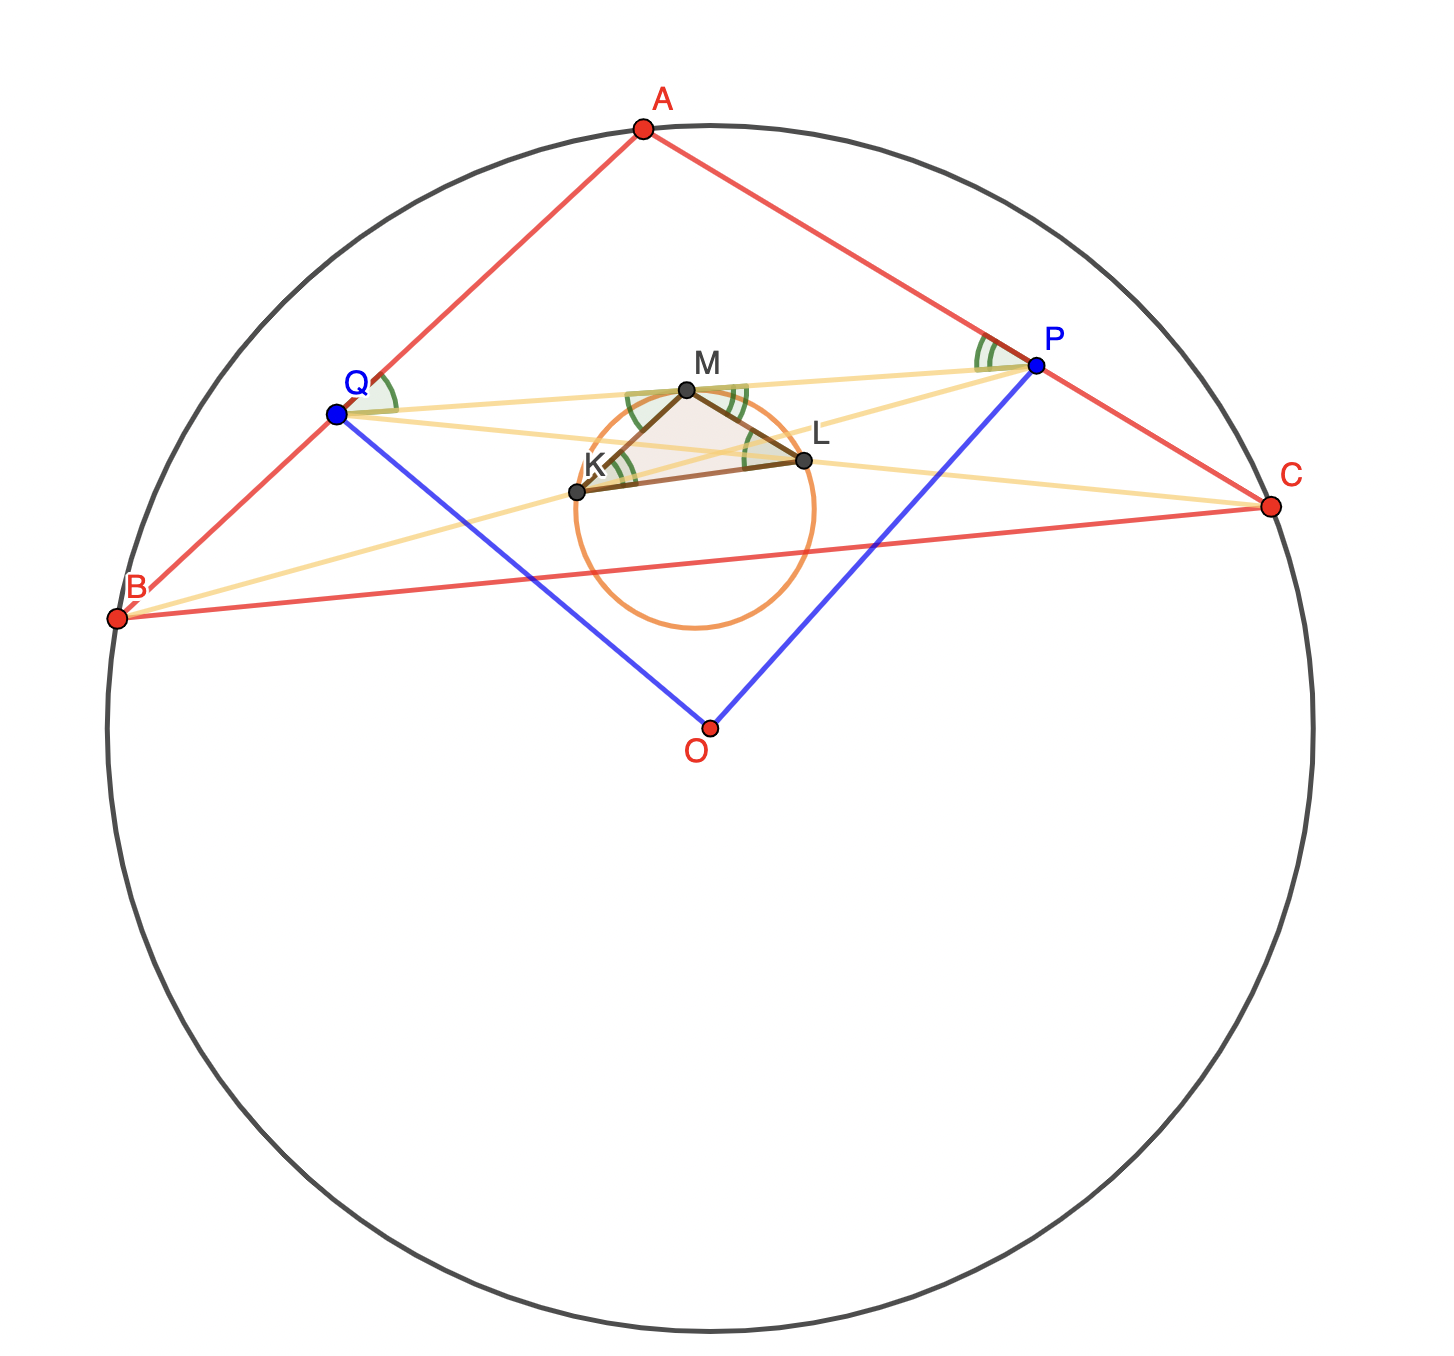
\includegraphics[scale=0.3]{IMO2009P2.png}\end{center}
\end{soln}
\begin{example}
  [USAMO 2012]
  Let $P$ be a point in the plane of $\triangle ABC$, and $\gamma$ a line passing through $P$. Let $A', B', C'$ be the points where the reflections of lines $PA, PB, PC$ with respect to $\gamma$ intersect lines $BC, AC, AB$ respectively. Prove that $A', B', C'$ are collinear.
\end{example}
\begin{soln}
  By Ratio Lemma,
  $$\frac{BA'}{A'C}\frac{CB'}{B'A}\frac{AC'}{C'B}=\left(\frac{BP}{CP}\frac{\sin \gamma}{\sin(2\alpha+\beta+\gamma)}\right)\left(\frac{CP}{AP}\frac{\sin\beta}{\sin\gamma}\right)\left(\frac{AP}{BP}\frac{\sin(2\alpha+\beta+\gamma)}{\sin\beta}\right)=1$$
  So we're done by Menelaus (Refer to the picture 2012AMOP5 in this directory).
\end{soln}
\begin{example}
  [ISL 2005]
  Given a triangle $ABC$ satisfying $AC+BC=3\cdot AB$. The incircle of triangle $ABC$ has center $I$ and touches the sides $BC$ and $CA$ at the points $D$ and $E$, respectively. Let $K$ and $L$ be the reflections of the points $D$ and $E$ with respect to $I$. Prove that the points $A$, $B$, $K$, $L$ lie on one circle.
\end{example}
\begin{soln}
  \begin{center}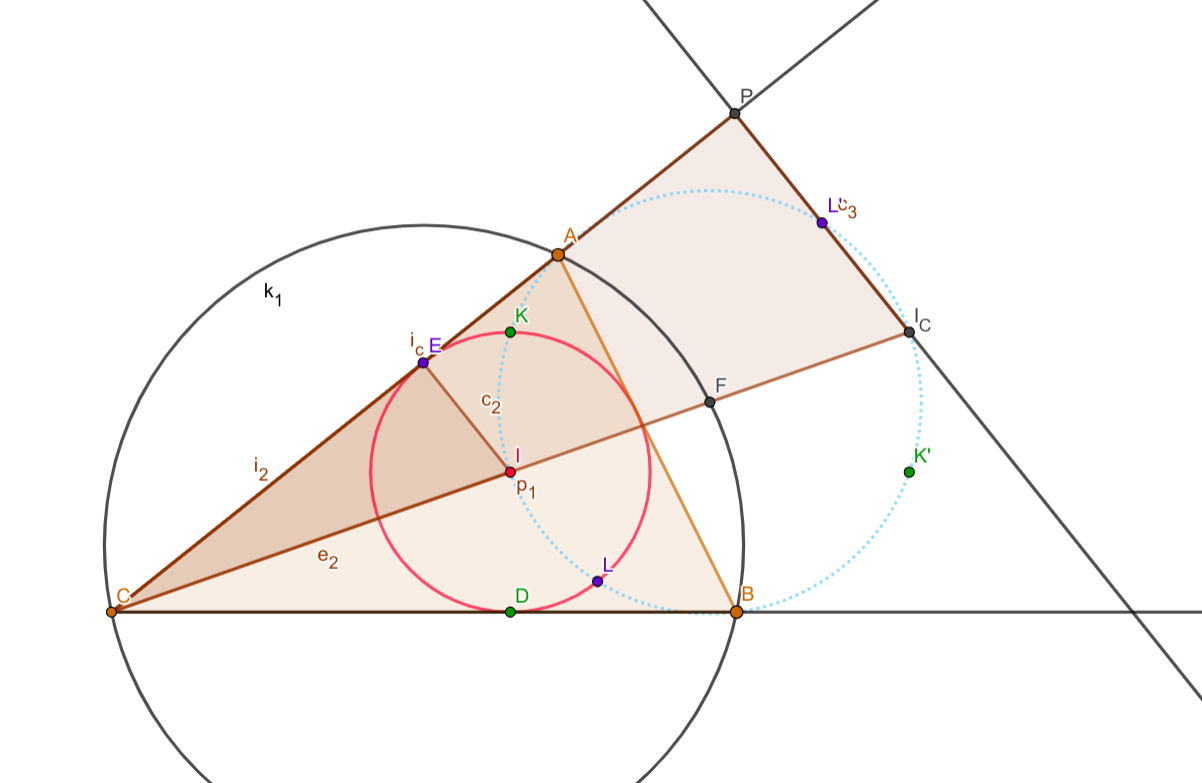
\includegraphics[scale=0.3]{image.png}\end{center}
    It's well known that $CE=s-c, CP=s$. But the length condition tells us that $c=\frac{s}{2}$, hence $\frac{CE}{CP}=\frac{1}{2}$. But $\triangle CIE\sim\triangle CI_CP$ by AA, so $CI=II_C$. Since $EI=LI$ and $\angle I_CIL=\angle EIC$ by vertical angles, $\triangle ILI_C\cong \triangle IEC$ by SAS. Hence $\angle IEC=\angle ILI_C=90$. But it's well known that $I,A,B,I_C$ are concyclic with $II_C$ as a diameter, so this condition implies that $L$ lies on $(IABI_C)$. By symmetry, $K$ does as well, so we're done.
\end{soln}
\begin{example}
  [USAMO 1974 P3]
  Two boundary points of a ball of radius 1 are joined by a curve contained in the ball and having length less than 2. Prove that the curve is contained entirely within some hemisphere of the given ball.
\end{example}
\begin{center}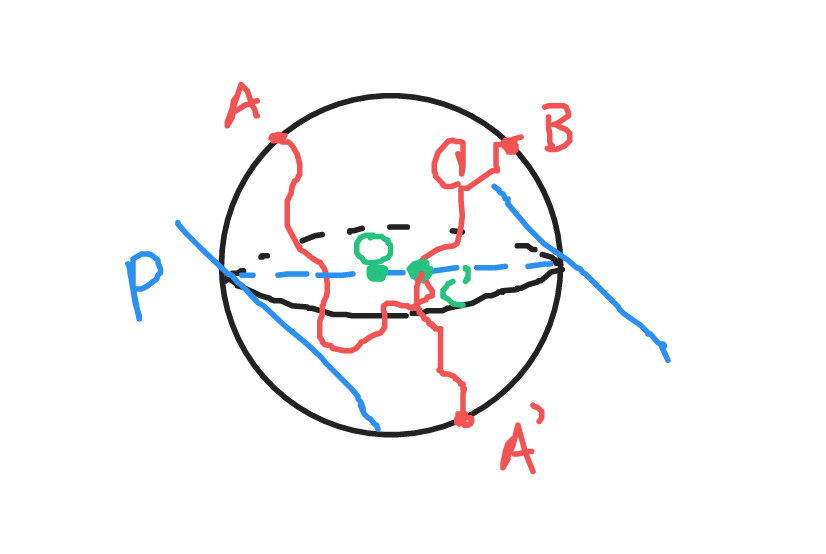
\includegraphics[scale=0.3]{USAMO1974P3.png}\end{center}
  \begin{soln}
    Suppose the two points are $A,B$, and the center of the sphere is $O$. Let $OA$ hit the circle for the second time at $A'$.
    Draw the plane $\mathcal{P}$ such that $\mathcal{P}\perp BA'$ and $O\in\mathcal{P}$ (which is uniquely determined by whatever property).
    I claim that the curve lies on one hemisphere of the sphere cut by $\mathcal{P}$, which is a much stronger formulation.
    Suppose otherwise, then the curve $\mathcal{C}$ hits $\mathcal{P}$ at $C'$. Reflect the part of $\mathcal{C}$ hitting $B,C'$ over to pass through $A',C'$.
    Length is preserved, so we just need to show that this reflection plus the other part of $\mathcal{C}$ has length greater than $2$.
    This is true since it takes $A$ to its diametrically opposite point, $A'$. \\ \\
    Note: This problem generalizes nicely, its an exercise to generalize and provide the proof.
  \end{soln}
  \begin{example}
    [Crux 4664]
    Let $ABCDEF$ be a cyclic hexagon such that $AD,BE,CF$ concur and
    $AB=CD=EF=\frac{AF+BC+DE}{3}$. Prove that it's a regular hexagon.
  \end{example}
  \begin{soln}
    Suppose that $AD,BE,CF$ concur at $O$. Angles $\angle ABO,\angle EDO$ are equal since they both subtend arc $AE$. By vertical angles, $\angle AOB=\angle EOD$, hence $\triangle ABO\sim\triangle EDO$. Thus
    $$\frac{AB}{DE}=\frac{AO}{EO}$$
    Analogously,
    $$\frac{CD}{AF}=\frac{CO}{AO}$$
    $$\frac{EF}{CB}=\frac{EO}{CO}$$
    Hence
    $$\frac{AB\cdot CD\cdot EF}{CB\cdot AF\cdot DE}=1$$
    Since $AB=CD=EF=\frac{CB+AF+DE}{3}$, we have that
    $$\frac{CB+AF+DE}{3}=\sqrt[3]{CB\cdot AF\cdot DE}$$
    However, the AM-GM inequality tells us that
    $$\frac{CB+AF+DE}{3}\ge \sqrt[3]{CB\cdot AF\cdot DE}$$
    with equality at $CB=AF=DE$. Thus all the sides are equal and the hexagon is regular.
  \end{soln}
\end{document}

